%%----------- 
\chapter{Introdução} %--- Capítulo 1
\thispagestyle{empty}
%%-----------

Atualmente, o ramo de impressoras 3D cresce a cada ano e se consolida cada vez mais como o próximo aparelho que as pessoas desejarão ter em casa. Os objetos fabricados nesses tipos de impressoras já conseguem atingir resoluções em algumas centenas de nanômetros e as utilizações se tornam cada vez mais baratas.

Em contrapartida, o escaneamento de objetos para uma modelagem tridimensional cresce moderadamente apresentando uma perspectiva de 15\% de crescimento nos próximos cinco anos, possuindo atualmente os scanners portáteis como maiores influenciadores desse crescimento \cite{creaform_ebooks_introduction_2015}. 

% ---
\section{Aplicações mais comuns de Escaneamento Tridimensional}
% ---

As aplicações do escaneamento de objetos são várias, mas destacam-se:

\begin{itemize}
\item \textbf{Engenharia reversa}: reconstruindo objetos;

\item \textbf{Controle de qualidade, análise e documentação}: utilizando técnicas de análise CAI (Computer-aided Inspection) e análises CAE (Computer-aided engineering);

\item \textbf{Arquitetura}: modelando construções objetos e monumentos históricos com o propósito de remodela-los;

\item \textbf{Multimídia}: com a rápida construção de modelos tridimensionais para jogos e  filmes;

\item \textbf{Artes}: com a digitalização de esculturas e outros patrimônios culturais;

\item \textbf{Medicina}: na reconstrução e visualização de partes do corpo humano, com o intuito de enxergar anomalias.
\end{itemize}

% ---
\section{Classificações de \textit{Scanners} 3D}
% ---

Podem-se estabelecer alguns critérios para classificação de \textit{scanners} 3D, tais como o método de construção/utilização, ou ainda quanto ao método de escaneamento. Assim, quanto ao método de construção/utilização, os \textit{scanners} 3D podem ser divididos em:

\begin{itemize}
\item \textbf{Estacionários}: estão fixos em apenas uma localização, geralmente sendo usados para escaneamento de largas proporções;

\item \textbf{Móveis}: que possuem a vantagem de serem menores, sendo usualmente utilizados no escaneamento de objetos imóveis e de proporções medianas e pequenas.
\end{itemize}

Quanto aos métodos de escaneamento os \textit{scanners} 3D se dividem basicamente em:

\begin{itemize}
\item \textbf{Com contato}: é necessário um contato mecânico com o objeto, e geralmente são estacionários, pois necessitam de uma referência de posição inicial. Um exemplo comum desse tipo são máquinas do tipo CMM (coordinate measuring machines);

\item \textbf{Sem contato}: Utilizam sensores ópticos, lasers e outras tecnologias de escaneamento. 
\end{itemize}

% ---
\section{Principais Tipos de Tecnologias de Escaneamento Tridimensional}
% ---

Esmiuçando-se os métodos de escaneamento pode-se falar mais especificamente das tecnologias empregadas em cada um dos métodos mais conhecidos. Assim, podem-se empregar raios-x de maneira controlada para aplicações médicas, como numa tomografia, por exemplo, ou utilizar ultrassom em técnicas sem contato e \textit{scanners} mecânicos em técnicas com contato, ou ainda, é possível modelar completamente objetos, destruindo-os em camadas, com o propósito de também modelá-los internamente \cite{toth_comparison_2014}.

Para aplicações sem contato e sem serem intrusivas, diferentemente dos raios-x, tem-se que as principais técnicas de escaneamento de objetos são: Fotogrametria (\textit{Photogrammetry}), Triangulação com Laser (\textit{Laser Triangulation}), Luz Estruturada (\textit{Structured Light}) e Tempo de Voo (\textit{Time-of-flight}). A seguir, essas técnicas serão explicadas um pouco mais detalhadamente.

%%-----------------------------
\subsection{Fotogrametria (\textit{Photogrammetry})}
%%-----------------------------

Foi a primeira técnica a ser pensada pelos cientistas, logo após a invenção da fotografia. A ideia básica consiste em tentar imitar a visão humana, usando várias imagens tiradas do objeto de diferentes posições, permitindo assim, medir e determinar a localização espacial do objeto. Esse processo também é chamado de triangulação. 

Hoje em dia a técnica ainda é amplamente usada principalmente na construção de mapas e imagens iterativas, uma vez que, não necessita de um aparato de hardware especial, com apenas uma câmera simples em um \textit{smartphone}, é possível recriar um cenário tridimensionalmente. Na figura \ref{fig-cap1-foto} é mostrada uma analogia do procedimento de fotogrametria. 

Um exemplo bastante evidente da técnica é a ferramenta \textit{Google Street View}, na qual um carro circula pela localização tirando várias fotos enquanto trafega, em todas as direções, que posteriormente serão interpoladas e transformadas num mapa iterativo do local fotografado.

\begin{figure}[H]
	\begin{center}
		\caption{Exemplo demonstrativo do uso da Fotogrametria.}		
		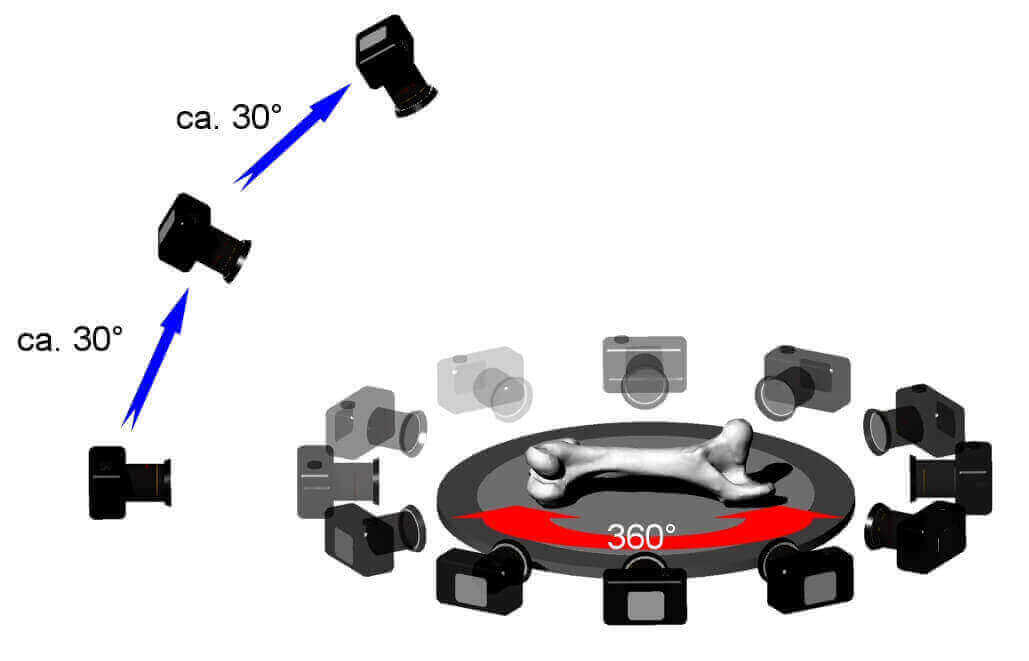
\includegraphics[width=\textwidth]{figs/cap1-foto.jpg}
		\legend{Fonte: extraída de \cite{noauthor_best_nodate}}
		\label{fig-cap1-foto}
	\end{center}
\end{figure}

%%-----------------------------
\subsection{Triangulação com Laser (\textit{Laser Triangulation})}
%%-----------------------------

O método de triangulação com laser é baste similar ao da fotogrametria ou da luz estrutura, uma vez que, todos esses utilizam o mesmo princípio geométrico de medição de distâncias entre referências e sensores. Os \textit{scanners} 3D com laser projetam um feixe de laser no objeto e a câmera pertencente ao dispositivo captura onde o feixe encostou-se ao objeto. Uma vez que as medidas de distância e os ângulos entre o feixe e a câmera são bem conhecidos, pode-se estimar com bastante precisão a localização do ponto ou linha de laser no objeto.

Os \textit{scanners} desse tipo geralmente são bem precisos e possuem resolução de até algumas dezenas de micrômetros. Em contra partida, o alcance do laser, usualmente, não ultrapassa alguns centímetros, e é mais difícil encontrar modelos portáteis utilizando essa tecnologia. Na figura \ref{fig-cap1-laser} é apresentado um esquema da aquisição e de uma possível saída no uso da técnica de triangulação com laser \cite{wispel_um_2017}\cite{pawar_review_2017}.

\begin{figure}[H]
	\begin{center}
		\caption{Aquisição e saída de \textit{scanner} utilizando triangulação com laser.}		
		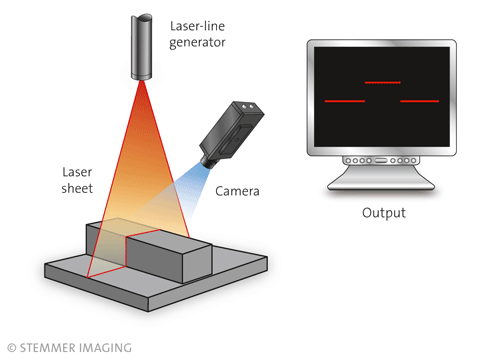
\includegraphics[scale=0.8]{figs/cap1-laser.png}
		\legend{Fonte: extraída de \cite{noauthor_3d_nodate-1}.}
		\label{fig-cap1-laser}
	\end{center}
\end{figure}

%%-----------------------------
\subsection{Luz Estruturada (\textit{Structured Light})}
%%-----------------------------

Para esse tipo de tecnologia, os dispositivos possuem algum tipo de projetor (RGB ou infravermelho, geralmente) que projetam um determinado padrão de imagem já previamente mapeado e calibrado. Uma vez que ao encostar-se a um objeto, o padrão é distorcido, tem-se que é possível determinar a localização de cada um dos pontos. 

Geralmente se utilizam mesas giratórias para fazer o objeto girar enquanto a captura está sendo feita, ao mesmo tempo em que se junta às diversas nuvens de pontos adquiridas. \textit{Scanners} desse tipo, assim como os de triangulação com laser, também são extremamente precisos e com altas resoluções, chegando até algumas dezenas de micrômetros \cite{lilienblum_structured_2015}. 

Embora o método de escaneamento seja parecido, os \textit{scanners} utilizando luz estruturada são menos nocivos aos seres humanos que os de laser, uma vez que, o feixe utilizado nesses podem chegar a cegar. Além disso, a grande maioria dos \textit{scanners} portáteis utiliza essa técnica. Na figura \ref{fig-cap1-struct}, é mostrada a relação geométrica entre o projetor dos padrões, a câmera de aquisição de imagem e o objeto escaneado \cite{geng_structured-light_2011}.

\begin{figure}[H]
	\begin{center}
		\caption{\textit{Setup} de utilização da técnica de Luz Estruturada.}		
		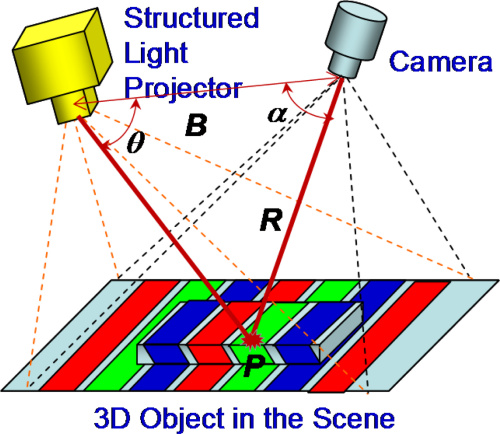
\includegraphics[scale=3]{figs/cap1-struct.jpg}
		\legend{Fonte: extraída de \cite{geng_structured-light_2011}.}
		\label{fig-cap1-struct}
	\end{center}
\end{figure}

%%-----------------------------
\subsection{Tempo de Voo (\textit{Time of Flight}, TOF)}
%%-----------------------------

Esses tipos de \textit{scanners} são, talvez, os que empregam a tecnologia mais desafiadora e ao mesmo tempo mais potencialmente recompensadora de todas as já mencionadas. Isso porque, o princípio básico desse \textit{scanner} é o de mandar um feixe de laser até o objeto através de um emissor, e calcular o tempo total até a reflexão baseado no que é recebido pelo receptor do dispositivo.

Considerando que a luz do sol demora apenas 8 minutos e 17 segundos para chegar a Terra, numa distância de 149 600 000 de quilômetros, pode-se imaginar o quão precisos devem ser os sensores desses dispositivos. Assim, os melhores dispositivos que existem hoje em dia e que empregam essa técnica, ainda não conseguem respostas tão precisas quanto os que utilizam as outras técnicas já mencionadas. Na figura \ref{fig-cap1-tof} é possível observar uma representação do esquema geral de funcionamento do TOF.

Um exemplo que utiliza a técnica é a segunda e mais nova versão do \textit{Kinect} da \textit{Microsoft}, utilizado no \textit{Xbox One}, que é um sensor de proximidade e captura de movimentos. Diferentemente da primeira versão que usava a técnica de luz estruturada, por meio de um projetor e câmera infravermelhos, o mais novo se utiliza do TOF.

\begin{figure}[H]
	\begin{center}
		\caption{Funcionamento geral da técnica Tempo de Voo.}		
		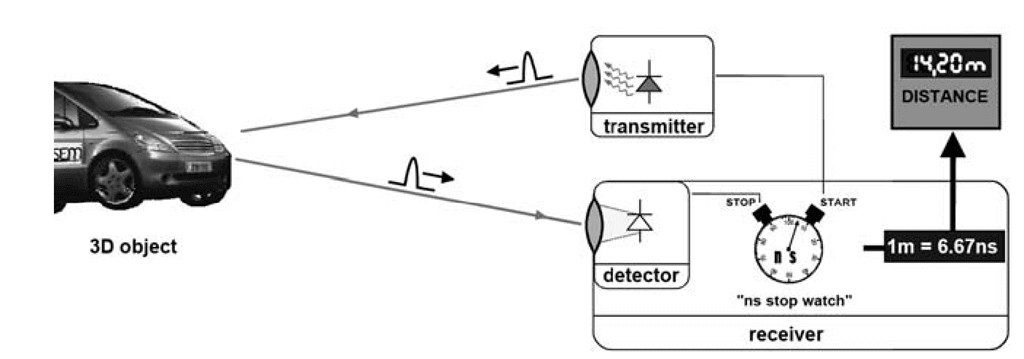
\includegraphics[width=\textwidth]{figs/cap1-tof.png}
		\legend{Fonte: extraída de \cite{noauthor_3d_nodate}.}
		\label{fig-cap1-tof}
	\end{center}
\end{figure}
